\documentclass{article}
\usepackage[utf8]{inputenc}
\usepackage{graphicx}
\usepackage{hyperref}
\usepackage{framed}
\usepackage{rotating}
\usepackage{tabularx}
\usepackage{tabu}
\usepackage{booktabs}% for better rules in the table
\usepackage{pgfplots}
\usepackage{adjustbox}
\usepackage{anyfontsize}
\newcommand{\changefont}[3]{\fontfamily{#1} \fontseries{#2} \fontshape{#3} \selectfont}


\pgfkeys{/pgfplots/MyAxisStyle/.style={xmin=0,xmax=3906, ymin=0,ymax=7000,height=4cm,width=0.9\linewidth,scale only axis}}

\usepackage{environ}
\makeatletter
\newsavebox{\measure@tikzpicture}
\NewEnviron{scaletikzpicturetowidth}[1]{%
  \def\tikz@width{#1}%
  \def\tikzscale{1}\begin{lrbox}{\measure@tikzpicture}%
  \BODY
  \end{lrbox}%
  \pgfmathparse{#1/\wd\measure@tikzpicture}%
  \edef\tikzscale{\pgfmathresult}%
  \BODY
}
\makeatother


% Debug graph font
% \font\nullfont=cmr10


%
% DONE:  SCALE + COLORS + TABLE
% TODO:  TEXT!!!
%


\begin{document}


\begin{titlepage}

\begin{center}
    \includegraphics{logo.jpg}\\[0.5cm]
    \textsc{\Large System and Network Engineering,MSc}\\[0.5cm]
    \textsc { \large Large Installation Administration}\\[1cm]
    { \Huge \bfseries Geographically Elastic Application \& Data Volume Migration Automation}\\[0.4cm]
    { \huge \bfseries DAFT: Docker, Ansible, Flocker Testing}\\[2cm] % Title of your document

\large Mathijs Houtenbos\\
\href{mailto:Mathijs.Houtenbos@os3.nl}{\texttt{Mathijs.Houtenbos@os3.nl}}\\[0.2cm]
\large Nikolaos Petros Triantafyllidis\\
\href{mailto:Nikolaos.Triantafyllidis@os3.nl}{\texttt{Nikolaos.Triantafyllidis@os3.nl}}\\[1cm]

\large \today

\end{center}

\end{titlepage}



\clearpage
\begin{abstract}
\noindent
This project deals with Application and Data Migration mechanisms over Docker containers. We propose and test a Data Migration scheme using Docker as our main software component, Flocker for cluster management and Ansible for configuration automation.\\
Our experiment consists of a MongoDB container that is migrated around the world trough Amazon Virtual Hosts in geographically remote locations. The purpose is to measure the downtime of the system during migration.\\
This report concludes that the proposed migration scheme is feasible and fairly simple but the underlying technology mature enough at this point of time. Moreover, we observe a good migration/downtime ratio but there is a lot of room for improvement. Finally, the system does not scale very well and because of the times and errors involved with larger data sizes it is not suitable for use with large production applications. \\
All the performed work and designed experiments as well as our results conclusions and suggestions are described in detail across this document.
\end{abstract}



\clearpage
\tableofcontents


\clearpage
\section{Introduction}
\textbf{Operating-system level virtualization} is a virtualization technique that calls for multiple isolated user spaces in a single Operating System, thus addressing issues such as performance overhead, flexibility and resource sharing \cite{os-level}.\\
In 2013 a new tool called Docker appeared aiming to extend existing OS level virtualization technologies, providing full toolchaining and automation for deploying applications in isolated execution environments called containers.\\
During its short lifetime Docker has managed to create a stable execution environment as well as a collaborative cloud platform. Docker is a well received technology \cite{Docker-usecases} that can be useful for both software developers and system administrators \cite{docker-whatis}.\\
\textbf{Dockerized} applications are very lightweight and are easily portable to any host that is capable of running the \textbf{Docker Engine}. Docker supports multi-container applications running on a single Docker host. These applications can have data volumes associated with them, which can be shared between containers \cite{docker-volumes}.\\
Docker, however, falls short when a multi-container application needs to run on a cluster of Docker nodes, with each of them running a different container. Moreover, the portability of the applications does not reflect to the data volumes as well. When a Docker container is moved its state is not moved with it \cite{flocker-article}.\\
This issue is addressed by a newly introduced tool called Flocker. Flocker promises easily deployable multi host Docker Cluster management as well as data migration over Docker containers.
The purpose of this research is firstly to test the feasibility of a Data Migration scheme using Docker containers managed with Flocker.\\
Secondly we will measure the downtime of the application and compare it with the total migration time in an attempt to determine the scalability of the migration scheme as the data volume grows in size.\\
Our last goal is to propose a fully automated procedure to harness the power of Docker combined with Flocker in the most transparent manner.\\
The rest of the chapter describes our main research question. The second chapter is dedicated to the description of the used software components. The third chapter describes the experimental setup and the execution of the measurements. The fourth chapter presents the results of the experiments and the fifth chapter summarizes our conclusions. Lastly the sixth chapter exhibits various obstacles that have held back our research and proposes future work.

\clearpage
\subsection{Research question}
The main research question that we will try to answer is the following:

\begin{itemize}
\item{Can we transparently migrate an application including data to where it is needed the most, and does this reduce latency?}
\end{itemize}

\subsubsection{Research question analysis}
The above research question can be analysed into the following more specific questions:
\begin{itemize}
\item{Is application migration \textbf{feasible} using this setup?}
\item{Is migration of an application done \textbf{transparently}, and on which levels?}
\item{How long does migration take, and is this \textbf{delay} acceptable?}
\item{Can applications be migrated automatically based on \textbf{geographical shifts} of clients and does this \textbf{reduce latency}?}
\end{itemize}



\clearpage
\section{Software Components}
Bellow is a brief description of all the software components that were used to conduct the experiements for this project. Besides Docker and Flocker that were introduced in the previous section we used Ansible as a configuration and automation component and a dockerized version of MongoDB acting as our data volume container. These tools were selected mainly because of their popularity and ease of use as well as their good integration with Docker.

\subsection{Docker}
\textbf{Docker} describes it self as an open platform for developers and sysadmins to build, ship, and run distributed applications \cite{docker-whatis}. \\
Docker operates by packaging applications together with their libraries and dependencies in lightweight isolated instances called \textbf{Software Containers}. Docker aims to extend Operating-System-Level Virtualization by providing extra layers of abstraction and automation \cite{docker-docs}.\\
Docker consists of two components; the \textbf{Docker Engine}, an open source container virtualization platform and \textbf{Docker Hub} a SaaS Cloud platform for sharing and managing Docker containers \cite{docker-components}.\\
Docker implements a client-server architecture. The Docker \textit{client} is the primary user interface that accepts commands from the user and interacts with the Docker \textit{daemon} which is responsible for building, running, and distributing Docker containers \cite{docker-architecture}.\\
Internally Docker distinguishes three distinct components, \textbf{Docker Images}, \textbf{Docker Registries} and \textbf{Docker Containers}.\\
A Docker image is described as a read-only template used to create containers. For example a Docker image can contain a base operating system a Web Server and a Web application. Docker provides a simple and straightforward toolchain for building images \cite{docker-inside}. Docker images consist of a series of layers combined into a single image with the use of \textbf{Union File Systems}. One of the performance advantages of Docker stems from the use of such layers. When a Docker image needs to be updated, a new layer containing the changes is built and instead of rebuilding and redistributing the whole image, that specific layer is only added or replaced\cite{docker-images}.\\
Docker registries are stores for Docker images, allowing users to push and pull existing images much like source code repositories\cite{docker-registries}. The aforementioned Docker Hub is the public Docker registry, used to share public Docker images between users \cite{docker-inside}.\\
Docker containers are created from Docker images. They are similar to directories in the sense that they hold everything that is needed for an application to run. Docker containers can be run, started, stopped, moved, and deleted \cite{docker-inside}. As has been mentioned before, Docker images are read-only. When a docker container is run a write-layer is added on top of the image, where the application can run\cite{docker-containers}.\\
Docker is written in Go and uses certain Linux kernel features to provide its functionality. Some of these features are first of all namespaces to provide with isolated workspaces for the containers, control groups (cgroups) to limit the usage of resources for each container, UnionFS for layer creation, etc. These components are compined into a wrapper called container format. The default container format is called \textit{libcontainer} and it is customly built for Docker \cite{docker-underlying}.\\[0.5cm]

\begin{center}
    \begin{figure}[h!]
    \centering
    \includegraphics[scale=0.5]{Docker-arch.png}
    \caption{Docker client-server architecture}
    \end{figure}
\end{center}

\subsection{Ansible}
\textbf{Ansible} is described as a free and Open Source IT automation tool used to configure systems, deploy software or orchestrate more advanced IT tasks such as continuous deployments or zero downtime rolling updates\cite{ansible-docs}.\\
Ansible is designed with simplicity and ease of use in mind. That is achieved via limitation of external dependencies and a language that is easily comprehensible even by users unfamiliar with the software and its inner workings. Ansible aims to be able to scale to any setup containing any number of machines ranging from one or two hosts to a few thousand servers\cite{ansible-docs}. \\
Ansible operates in an agentless and decentralized  manner. There is no Ansible deamon running on any Ansible-managed host as there is no dedicated Ansible server. Any machine that can install the Ansible command-line tools can manage hosts via Ansible. The mechanism used for transport is OpenSSH. Due to the decentralized nature of Ansible, authentication lies on existing OS credentials, such as SSH keys. If additional authentication measures are needed Ansible can be easily integrated with Kerberos and LDAP \cite{ansible-docs}. \\
Ansible can manage multiple machines in an infrastructure at the same time. This happens by selecting groups of machines defined in an inventory file that follows a format similar to an INI file.
Each group as well as each separate host can have a series of variables associated with them \cite{ansible-inventory}.\\
The software ships with a rich library of modules that are responsible for a number of tasks such as file management, database management, cloud management, networking, etc. Users can define their own Ansible modules, which are written in Python, and if the community guidelines are followed these modules can be included in the standard Ansible distribution \cite{ansible-modules}.
Modules can be run against hosts directly via the command line or through the configuration files that Ansible calls \textbf{Playbooks}.\\
Playbooks are described as the configuration, deployment, and orchestration language of Ansible. They can be used to describe certain policies that need to be enforced on remote systems, or simply a set of steps in a deployment process \cite{ansible-playbooks}.\\
Ansible playbooks are expressed in a YAML format and their syntax intentionally differentiates from a script but rather is a model definition.\\
Each playbook consists of one or more 'plays'. A play maps a group of hosts to certain well defined roles, represented simple tasks, that are basically calls to Ansible modules \cite{ansible-playbooks}. \\
For example, in a playbook with multiple plays one could run a series of tasks to all the webservers in an infrastructure then configure the database servers via another set of tasks and then return to the webservers to conclude the deployment of an application, and so on \cite{ansible-playbooks}.


\subsection{Flocker}
Flocker is described as a data volume manager and multi-host Docker cluster management tool. Its aim is to provide functionality for transferring databases, queues or key-value stores that run inside Docker containers as easily as any other stateless application, between different hosts. Flocker builds upon ZFS on Linux in order to deliver the desired functionality \cite{flocker-intro}.\\
While Docker can implement multiple containers running on a single node, even sharing their state over local disk volumes belonging to different containers, deploying a multi-node setup can introduce certain issues. Certain questions arise referring to the location of the containers, connecting to a container of interest, linking containers across different hosts, behavior of the state of an application during migration, etc. Flocker's purpose is to tackle these problems\cite{flocker-docks}.\\
First of all Flocker allows multiple containers to be deployed on a cluster of multiple nodes. It exposes an abstract configuration language that allows the user to define what containers they need to run on which hosts\cite{flocker-docks}.\\
Secondly, when it comes to networking Flocker configures containers to use externally visible TCP ports. Each host in the cluster implements the Flocker proxy what is responsible for redirecting network traffic to the node that hosts the appropriate container. That allows us to point an external domain name to all the nodes in the Flocker cluster and receive repsonse from our applications no matter which host receives the request\cite{flocker-docks}.\\
As far as application state is concerned Flocker attaches ZFS filesystems on Docker containers to serve as their Data Volumes. Flocker provides functionality for copying data volumes across hosts. Thus, if an application container is migrated to a different node Flocker automatically moves the volume associated with it\cite{flocker-docks}.\\
Flocker clusters are managed via two separate configuration files. The first is the Application Configuration file where the user describes the images that they need to include in each container. This is also the configuration file that includes volume mount points, networking ports and links and aliases through which the separate containers communicate\cite{flocker-docks}.\\
The second configuration file is called the Deployment Configuration file. This file simply lists all the hosts in a Flocker cluster and the containers that each node needs to host\cite{flocker-docks}.\\
Both these files follow a YAML syntax\cite{flocker-docks}.

\begin{center}
    \begin{figure}[h!]
    \centering
    \includegraphics[scale=0.3]{flocker-architecture-diagram.jpg}
    \caption{Flocker Architecture Diagram}
    \end{figure}
\end{center}

\subsection{MongoDB}
MongoDB is an open-source document oriented NoSQL database system. Its design goals include ease of development and scaling \cite{mongodb-docs}.\\
MongoDB stores schemaless key-value documents that follow a JSON object format.\\
One of its key features is high performance data persistence which is achieved via support for embedded data models that reduces I/O activity and indexing for faster queries that can include keys from embedded documents and arrays \cite{mongodb-intro}.\\
MongoDB also achieves high availability groups of database servers called replica sets that provide automatic failover and data redundancy \cite{mongodb-intro}.\\
Lastly MongoDB provides automatic scaling, via automatic sharding that distributes data across a cluster of machines and replica sets that provide eventually-consistent reads for low-latency high throughput deployments \cite{mongodb-intro}.\\
MongoDB provides all basic CRUD (Create, Read, Update, Delete) via a simple and straightforward querying language that is an extention of JavaScript\cite{mongodb-crud}.\\
Additionally MongoDB provides powerful Data Management and computation frameworks such as Aggregation Pipelines and Map-Reduce processing\cite{mongodb-aggregation}.

\clearpage
\section{Experiments}
The purpose of the experiment was to test the feasibility of the data migration scheme. Furthermore our aim was to measure the database downtime and compare it with the overall migration time and try to showcase that the database downtime is constant no matter how large the migrated volume is.

\subsection{Setup}
The first part of the experiment consisted of running Flocker locally on two Ansible-managed Fedora 20 hosts. The choice of the Operating System was simply because Flocker agent, in its current development state, is only supported on Fedora 20 hosts.\\
The purpose of the local setup was to familiarize ourselves with the setup of the Flocker agent on a host, get acquainted with the configuration of a Flocker cluster and examine the feasibility of the Data Migration process in a local environment. \\
On each Flocker host we run a 'Dockerized' web application written in Go, backed by a MongoDB in a separate container, that worked as our Data Volume.\\
The web application featured two very simple Web API calls used to insert and count the entries in the database, via HTTP POST and GET requests respectfully.\\
Both the Web Application and MongoDB Docker images that we created are publicly available on Docker Hub.\\
Table~\ref{tab:versions} show a summary of versions of all the software components used for this project.\\
All the obstacles that we had to overcome (more details on chapter 6) as well as all the basic settings we had to perform to create a stable working setup were captured in Ansible playbooks, to account for reproducible configuration.\\
This configuration was in turn deployed on four Amazon EC2 \cite{ec2} Virtual Machines located in four different geographical regions, namely EU (Ireland), US East (N.Virginia), US West (N. California) and Asia Pacific (Singapore).\\
The Flocker deployment and migration procedures were made possible by preparing an application manifest file that declared the Web Application and MongoDB containers together with their settings, as well as several deployment manifest files that declared the nodes on which each container would run.\\


\begin{table}[h]
    \centering
    \begin{tabular}{|c|c|}
    \hline
        Element & Version \\ \hline
        \textbf{Docker} & \\ \hline
        Client & 1.4.1 \\ \hline
        API & 1.16 \\ \hline
        Engine & 1.5.0 \\ \hline
        \textbf{Flocker} & 0.3.2\\ \hline
        \textbf{Ansible} & 1.8.4 \\ \hline
        \textbf{MongoDB} & 2.6.8 \\ \hline
        \textbf{Golang} & 1.4.2 \\ \hline
    \end{tabular}
    \caption{Software Component Versions}
    \label{tab:versions}
\end{table}


\subsection{Execution}

The connections to the flock nodes around the world are shown in figure~\ref{fig:world_map}. The line going around the world is the path taken by our migrating docker containers, and the dotted lines indicate the control connections from the central control node in Amsterdam. \\
First a test run is initiated from the control node in Amsterdam and starts by initializing a fresh empty MongoDB database on the first node in EU-west (Ireland), this server has the fastest access since the datacenter is directly connected trough the AMS-IX Internet exchange. The database is then filled with a predetermined amount of data to test the migration process with different data sizes. After this the docker containers including the MongoDB database are migrated west towards the nodes in US-east (California), US-west (Virginia), and Asia (Singapore). When connecting amongst the flock nodes themselves the traffic does not leave the Amazon AS so there is not much that can be said about the intermediate networks. When we connect from the control node in Amsterdam (to the public Amazon IP) we connect to US-east trough NorduNET, to US-west trough GTT, and to Singapore trough NorduNET and subsequently PCCW/BTN. From this information is is already obvious that Singapore has the least favourable connectivity from our central location. We performed measurements to determine the latency between flock nodes as well as the latency from out central control node to the flock nodes.\\
To get an insight about the downtime of the database service we have devised a measurement scheme that consists of a script that performs iterative writes to the database system via calls to the MongoDB container. Then we start migrating the database container to a different node inside the flock, which will eventually cause the database to go offline for a certain period of time. During this period the Web Application responds with error messages which we use to define the moment in time that the database has gone offline. Once the database container has been migrated to its new host the writing process resumes. Thus, we define the database downtime as the interval between the last write before the migration procedure and the first right after the migration has been completed. The writes are then confirmed by requesting a database count from the Web Application, confirming operation of both the database and Web Application containers, as well as the presence of test data in the database.

% World map
\begin{center}
\begin{figure}[!ht]
    \makebox[\textwidth][c]{
        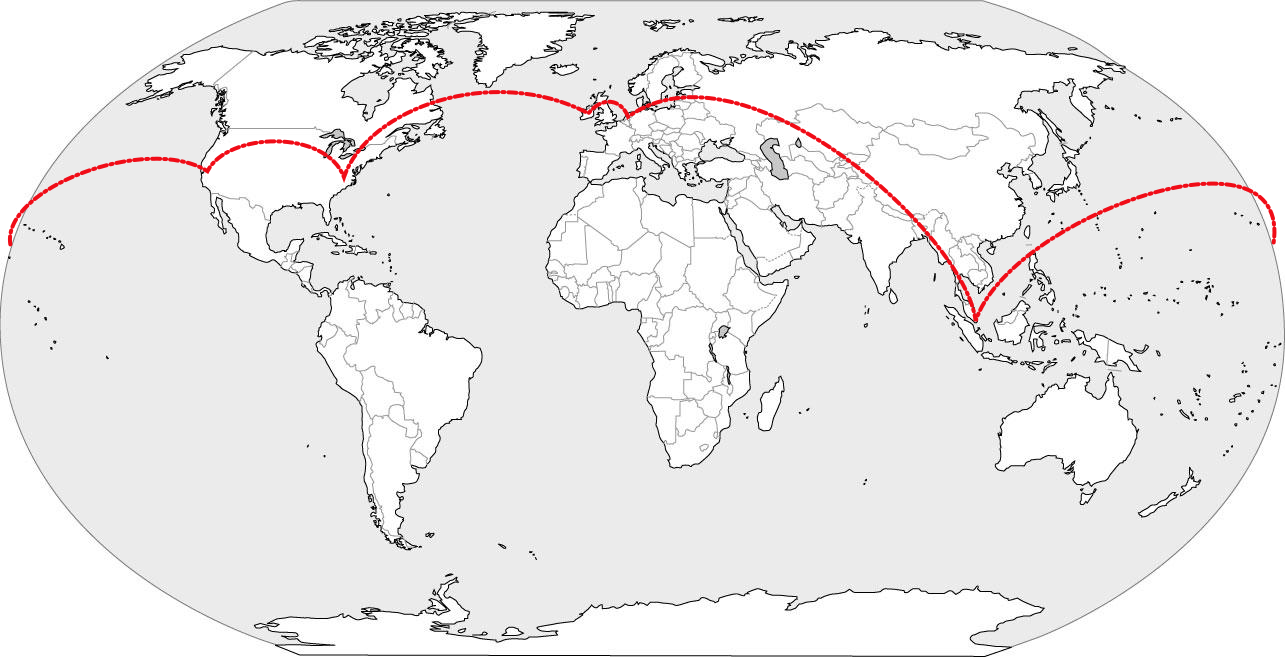
\includegraphics[width=1.2\textwidth]{around_the_world_without_amsterdam.png}
    }
    \caption{Worldmap showing the locations of our flock nodes and the centralized control from Amsterdam}
    \label{fig:world_map}
\end{figure}
\end{center}



\clearpage
\section{Results}
\subsection{Migration time and downtime}

We measured several metrics in relation the size of the database that was being migrated around the word. The graph in figure~\ref{fig:migration_size} shows the most important results from the size based measurements listed in table~\ref{tbl:size_data}. The most important result is that while the time for migration increases exponentially as can clearly be seen by looking at the trendline graph the downtime (when the application can not be reached, and no write operations can be performed) increases only slightly and in a linear fashion. The lowest migration time for an empty database took 116.71 s, and the downtime lasted 27.31 s on average, giving an initial downtime percentage of 34.04\%.
When transferring the largest database of 3906 MiB the migration lasted 6644.78 s, and the downtime lasted 225.53 s on average, giving a downtime percentage of 3.77\%. This relative decrease of downtime percentage can also clearly be seen in the graph.

% Line graph
\begin{center}
\begin{figure}[!ht]
    \makebox[\textwidth][c]{
        \includegraphics[width=1.5\textwidth]{Migration_time_compared_to_downtime_with_percentage.png}
    }
    \caption{Migration time compared to downtime in relation to database size}
    \label{fig:migration_size}
\end{figure}
\end{center}

Furthermore we measured for differences in downtime between the different region hops, and there is a clear difference visible in barchart in figure~\ref{fig:migration_region}. The migration time between US-east and US-west is almost half the migration time as observed between Asia and EU-west. The difference is explained by the increased distance, and thus higher latency. As can also be observed in table~\ref{tbl:region_data} the ping times between all the different regions flocker nodes are on average all below 150 msec, except the Asia region flocker node, which has a pint time of 200 msec from the other flocker nodes on average. This increased latency result in a slower migration between the two most distance flocker nodes, Asia and EU-west. This difference in latency of rougly 33\% results in an almost 100\% increase in migration time between the best and worst performing regions.

% Barchart
\begin{center}:
\begin{figure}[!ht]
    \makebox[\textwidth][c]{
        \includegraphics[width=1.4\textwidth]{Average_migration_time_compared_to_downtime_per_region.png}
    }
    \caption{Average migration and downtime per region hop}
    \label{fig:migration_region}
\end{figure}
\end{center}


\subsection{Transfer speed}

When measuring the transfer speed in relation to the size of the database an interesting pattern becomes clear as can be observed in the graph in figure~\ref{fig:transfer_size}. When migrating a very small database a large part of the migration time is spent on the overhead of the migration, resulting in a relatively long time to transfer a small amount of data, and thus a low average throughput over the whole migration. When the size of the database is increasing we observed the measurements reaching a peak where the average migration time is lowest compared the the amount of data, and thus a high throughput.\\
After this peak the transfer speed decreases on average. The most likely explanation is the increased overhead, when performing a large amount of write operations on the migrating database while performing a live migration. As is shown later the number of writes per second does not increase, but the longer duration of the transfer results in a higher amount of writes for each live migration copy iteration, most likely resulting in more iterations and thus an increase overhead.
The highest measured peak transfer speed was 2242 kbps for a database size of 703 MiB, and the best fitting trendline projects the peak transfer speed optimum around this database size. The largest database size of 3906 MiB has an average transfer speed of 750 kbps, which is only 33.5\% of the highest average speed. See table~\ref{tbl:size_data} for all other measurements.

% Line graph
\begin{center}
\begin{figure}[!ht]
    \makebox[\textwidth][c]{
        \includegraphics[width=1.5\textwidth]{Transfer_speed.png}
    }
    \caption{Transfer speed in relation to database size}
    \label{fig:transfer_size}
\end{figure}
\end{center}

As expected from earlier results there is also a clear difference in transfer speed per region hop as can be observed in the barchart in figure~\ref{fig:transfer_region}. All these connections are over Amazon networks, and because of this we can not measure any difference in number of hops with traceroute. The measured ping times between the different regions flocker nodes offer some explanation of this difference per region, but not entirely. An interesting difference is the transfer speed going into Asia is lower than the transfer speed going out of Asia. This is most likely a measurement error because of the high amount of errors observed in the Asia region flocker node. See table~\ref{tbl:region_hop_data} for all other measurements.

\begin{center}
\begin{figure}[!ht]
    \makebox[\textwidth][c]{
        \includegraphics[width=1.4\textwidth]{Average_transfer_speed_per_region.png}
    }
    \caption{Average transfer speed per region hop}
    \label{fig:transfer_region}
\end{figure}
\end{center}


\subsection{Application operation during migration}

During the migration the amount of write operations that were performed continually slowly decreased when the database size increased, as is illustrated in figure~\ref{fig:write_operations}. This decrease in write speed is a direct result of the increased overheads involved, both for writing data to a larger database (which can have multiple reasons, for example indexes and journaling \cite{mongodb-growth}), as well as the additional overhead involved when performing a large amount of write operations during live migration. The amount of write operations in the graph closely resembles the amount of time the migration takes (as shown in figure~\ref{fig:migration_size}), which also increases exponentially with the size of the database. Because the amount of writes per seconds only decreases linearly it follows that the number of write operations is only a slightly less steep exponential curve than the migration time.

% Line graph
\begin{center}
\begin{figure}[!ht]
    \makebox[\textwidth][c]{
        \includegraphics[width=1.5\textwidth]{Writes_per_second.png}
    }
    \caption{Write operations performed in relation to database size}
    \label{fig:write_operations}
\end{figure}
\end{center}


\subsection{Application performance after migration}

The graph in figure~\ref{fig:latency_size} shows the timings of the application response latency after the migration is completed the database is queried again trough the GO HTTP application. With an empty database the average time to get an HTTP response takes about twice the average time to connect to the HTTP server. This is expected because two round-trips are needed to request and receive an HTTP response. The time to connect is closely tied to the network latency and remains roughly the same for all different database sizes. The time to receive a response however slowly increases beyond the 2 × network round-trip latency you would expect as the database size increases, indicating that MongoDB becomes slightly less efficiënt when performing an count function on a larger database (which is of course expected of aggregate functions \cite{mongodb-aggregation}). The average application request query response latency increases the most from a minimum of 350 msec to a maximum of 410 msec, which implies an increase of 60 msec for MongoDB processing when the database is embiggened by 3203 MiB, as can be seen in table~\ref{tbl:size_data}.

% Line graph
\begin{center}
\begin{figure}[!ht]
    \makebox[\textwidth][c]{
        \includegraphics[width=1.5\textwidth]{Connect_latency.png}
    }
    \caption{Connection and query latency in relation to database size}
    \label{fig:latency_size}
\end{figure}
\end{center}

Of all the measurements the latency is the most pronounced different metric between the different regions as is illustrated in figure~\ref{fig:latency_region}. The total query latency listed in table~\ref{tbl:region_data} increases from the minimum of 74 msec in EU-west to a maximum of 741 in Asia, a tenfold difference in average application request query response latency.

% Barchart
\begin{center}
\begin{figure}[!ht]
    \makebox[\textwidth][c]{
        \includegraphics[width=1.4\textwidth]{Connect_latency_per_region.png}
    }
    \caption{Average connection and query latency per region}
    \label{fig:latency_region}
\end{figure}
\end{center}


\subsection{Measurement errors}

A lot of the (still fairly small) measurement errors in the aforementioned results becomes apparent when we diagnosed the (lack of) returned data from our tests. As can be seen in the barchart in figure in figure~\ref{fig:errors_region} more than 10\% (partial) failures resulting in either database timeout or a complete migration failure. The chances of a failure increase most when migration from Asia to EU-west, which is also the region hop with the highest latency, a low transfer speed, but most importantly the longest average migration times. The software used appears not to be very fault tolerant resulting in a large amount of (partial) measurement errors. The exact amount of errors is listed in table~\ref{tbl:region_hop_data}.

% Barchart
\begin{center}
\begin{figure}[!ht]
    \makebox[\textwidth][c]{
        \includegraphics[width=1.4\textwidth]{Migration_errors_per_region.png}
    }
    \caption{Migration measurement success and errors per region}
    \label{fig:errors_region}
\end{figure}
\end{center}




\clearpage
\section{Conclusions}

Using Flocker to migrate an application which consists of multiple Docker containers including a database and controlling the process with Ansible \textbf{is feasible}, but only in a limited set of circumstances. It requires a specific server setup with Fedora 20, with a specific kernel to support ZFS, and preferably a local network connection with low latency connecting the flocker nodes. These restrictions make it practically infeasible for the goals we originally set, but in the course of this project we redefined the goals to a potentially feasible subset with the constraints set by the software used. \\ \\

The application has \textbf{fairly good location transparency} during normal operation and during live migration which means it also has \textbf{good migration transparency}. When querying any one flocker node the result is almost always returned by means of the docker-proxy that forwards the request to the flocker node currently running the application.
The downtime at the end of a live migration could be seen as \textbf{bad relocation transparency}. This is caused by the low average transfer speeds result in very long migration times when the database size increases, and while the downtime does not increase nearly as much as the migration time it is still a relatively long time with the average well over a minute (69.51 s).
But connection issues sometimes prevented the connection which resulted in \textbf{unreliable network transparency}, so while the docker-proxy works very well in ideal scenario's it fails to offer fault tolerance on the network level. This also indicates the application had \textbf{no fully matured failure transparency}.
The application also has \textbf{excellent security transparency}, all the software used is distributed freely online. Beside basic OS configuration the application requires no additional security measures and was openly available (from the OS3 network and the Amazon flocker nodes). \\ \\

\textbf{Migration takes much too long}, and the migration time does not scale. Where the 1172 MiB database still took only 11 minutes the 3906 MiB database already takes 111 minutes! And while the downtime does not increase exponentially like the migration time is still increases from less than 30 s for databases smaller than 300 MiB to over 225 s for the 3906 MiB database. These migration times and downtimes are unacceptable for most applications, and when the application database size must scale to sizes bigger than 4 GiB this becomes unworkeable. Bigger databases will take hours or days to migrate, and the high error rate practically guarantees that these migrations will fail. Beside the increasing time to migrate the application data the writes per second decreased during migrations as the database size increased. When migrating large databases this will become another issue with scaling, resulting in a barely useable applcation during migration. \\ \\

This mechanism to migrate applications could potentially be used to migrated automatically based on geographical shifts of clients, but methods for automating this based on actual measurements was outside the scope of this project because of time and technological restrictions. The \textbf{high potential to reduce latency} however is proven by our measurements. The tenfold decrease of latency when migration the application from Asia to EU-west improves the latency from 741 msec to only 74 msec. In a real world interactive application this difference huge, the 74 msec being a hardly noticeable delay and the 741 msec begin a nuisance which will certainly result in a loss of clients \cite{google_msec}. \\ \\

Lastly the software used is too unstable to use in production (which is clearly stated on the Flocker site). This unstable software lead to many configuration problems and incompatibilities, and once up and running still had more than 10\% (partial) failures resulting in either database timeout of complete migration failure. We do not recommend using this software for anything other than small-scale research projects. \\ \\


\clearpage
\section{Obstacles \& Future Work}
\subsection{Obstacles}
As it has been mentioned before we run into several problems during the setup phase that obstructed our research.\\
First of all our initial designed called for a heterogeneous cluster of local VMs running different operating systems, in an attempt to showcase the cross-platform power of Docker. The case, however, is that Flocker Node, the agent responsible for Flocker cluster deployment on each host runs only on Fedora 20 in the current development phase of the tool. The command line tools for Flocker can run on Debian-based or RedHat-Based Linux nodes and even OS X machines, a fact that is advertised strongly on the main Web page of the tool\cite{flocker-page}. One would, however, need to thoroughly go through deeper levels of documentation to be informed that Flocker Node only runs on one specific version of a particular Linux Distribution.\\
Moreover we also had to drop the virtualization approach since Fedora 20 is not supported on Xen, the virtualization platform running on our dedicated OS3 servers \cite{Xen}.\\
We installed a minimal version of Fedora 20 on two bare metal servers. The first problem we had to tackle was the fact that in this distribution even the most basic Networking tools like ifconfig and traceroute were absent, which make network configuration much more time consuming than it should be.\\
Following the official installation guide for Flocker on Fedora 20 \cite{flocker-install}, we managed to setup the Flocker agent on our server nodes. However, deployment of any container setup under Flocker was not possible. This is because ZFS, a very basic dependency of Flocker, could not be built on Linux kernel version 3.18, the kernel version mentioned in the official documentation of the tool. In order for this to be circumvented the kernel of the machines had to be downgraded to kernel version 3.16, a version that is not present in the official software repositories.\\
After we managed to correctly install Flocker Node and its dependencies, we tried again to deploy our setup with both Web Application and MongoDB containers running on the same host. The problem we saw at this point was that while the Web Application was functioning well, the MongoDB was terminating after a few seconds. We discovered that this was due to Docker not interacting well with SeLinux, which was then disabled.\\
The next issue we encountered was that while each container was able to communicate with the outside world seamlessly, simply by defining a communication port in the application manifest file that Flocker reads, they cannot talk to each other even if they are running on the same host. Flocker builds on Docker's functionallity of linking containers together. This happens simply by defining internal and external links in the Application manifest file of Flocker. These links work by populating certain environmental variables inside all the containers that form a Flocker cluster. For these reason the Web Application had to be re-written and re deployed inside a Docker container, at this point, to make use of these specific variables. Even after this setup, however, links were not able to work without disabling the firewall.\\
A lof of the problems mentioned before stem from incomplete documentation of our main component Flocker. For example the issue with the kernel version is not mentioned in the installation guide and it was discovered due to a coincidental comment by one of the Flocker users \cite{flocker-install}. Furthermore, the deployment examples provided in the official documentation demonstrate some basic use cases and present certain features of the tool, fail, however, to show how these examples can be generalized and tailored to the needs of each application.


\subsection{Future Work}
It becomes apparent this attempt is preliminary at this stage and that there is a lot of work still to be carried out in the field of data migration using Docker containers.\\
First of all once the underlying technology has matured enough to provide more stable execution environments the present research could be revisited and new measurements could be performed, even with larger data volumes, to produce more reliable results.\\
As it has been mentioned before, Flocker currently only works for one specific Linux distribution. Once the technology has been expanded to other platforms as well it would be very interesting to repeat the present research in a heterogeneous environment and compare the results.\\
The process we have described is automated to some degree. It would be, nonetheless, useful to create a full automation scheme via a single orchestration tool like Ansible, whose functionallity could be extended to include modules for the management of Flocker clusters.\\
Lastly an analytics platform such as the ELK stack (Elasticsearch, Logstash, Kibana)\cite{elk} could provide useful insights about the usage and the stress of each node inside the Flocker cluster, information that could be used to trigger data migrations, responding to usage details.


\clearpage
\begin{thebibliography}{99}
\bibitem{os-level}
Yu, Y. (2007). OS-level Virtualization and Its Applications. Ph.D. Stony Brook University.
\url{http://www.ecsl.cs.sunysb.edu/tr/TR223.pdf}
\bibitem{Docker-usecases}
Docker.com, (2015). Use Cases - Examples | Docker. [online] Available at: \url{https://www.docker.com/resources/usecases/}
\bibitem{docker-whatis}
Docker.com, (2015). What Is Docker? An open platform for distributed apps. [online] Available at: \url{https://www.docker.com/whatisdocker/}
\bibitem{docker-volumes}
Docs.docker.com, (2015). Managing data in containers - Docker Documentation. [online] Available at: \url{https://docs.docker.com/userguide/dockervolumes/}.
\bibitem{flocker-article}
Yegulalp, S. (2015). Docker gains migration and networking help with Flocker. [online] InfoWorld. Available at: \url{http://www.infoworld.com/article/2849242/application-virtualization/docker-gains-migration-and-networking-help-with-flocker.html}.
\bibitem{docker-docs}
Docs.docker.com, (2015). Managing data in containers - Docker Documentation. [online] Available at: https://docs.docker.com/userguide/dockervolumes/ [Accessed 3 Apr. 2015].
Docs.docker.com, (2015). Docker Documentation. [online] Available at: \url{https://docs.docker.com}
\bibitem{docker-components}
Docs.docker.com, (2015). Understanding Docker - Docker Documentation. [online] Available at:
\url{https://docs.docker.com/introduction/understanding-docker/#what-are-the-major-docker-components}
\bibitem{docker-inside}
Docs.docker.com, (2015). Understanding Docker - Docker Documentation. [online] Available at: \url{https://docs.docker.com/introduction/understanding-docker/#inside-docker}
\bibitem{docker-architecture}
Docs.docker.com, (2015). Understanding Docker - Docker Documentation. [online] Available at:
\url{https://docs.docker.com/introduction/understanding-docker/#what-is-dockers-architecture}
\bibitem{docker-images}
Docs.docker.com, (2015). Understanding Docker - Docker Documentation. [online] Available at: \url{https://docs.docker.com/introduction/understanding-docker/#how-does-a-docker-image-work}
\bibitem{docker-registries}
Docs.docker.com, (2015). Understanding Docker - Docker Documentation. [online] Available at: \url{https://docs.docker.com/introduction/understanding-docker/#how-does-a-docker-registry-work}
\bibitem{docker-containers}
Docs.docker.com, (2015). Understanding Docker - Docker Documentation. [online] Available at: \url{https://docs.docker.com/introduction/understanding-docker/#how-does-a-container-work}
\bibitem{docker-underlying}
Docs.docker.com, (2015). Understanding Docker - Docker Documentation. [online] Available at: \url{https://docs.docker.com/introduction/understanding-docker/#the-underlying-technology}
\bibitem{ansible-docs}
Docs.ansible.com, (2015). Ansible Documentation — Ansible Documentation. [online] Available at:
\url{http://docs.ansible.com}.
\bibitem{ansible-inventory}
Docs.ansible.com, (2015). Inventory — Ansible Documentation. [online] Available at: \url{http://docs.ansible.com/intro_inventory.html}
\bibitem{ansible-modules}
Docs.ansible.com, (2015). About Modules — Ansible Documentation. [online] Available at: \url{http://docs.ansible.com/modules.html}
\bibitem{ansible-playbooks}
Docs.ansible.com, (2015). Playbookss — Ansible Documentation. [online] Available at: \url{http://docs.ansible.com/playbooks.html}
\bibitem{flocker-page}
Docs.clusterhq.com, (2015). Getting started with Flocker — Flocker 0.3.2 documentation. [online] Available at: \url{https://docs.clusterhq.com/en/0.3.2/gettingstarted/}.
\bibitem{flocker-install}
Docs.clusterhq.com, (2015). Installing Flocker. [online] Available at: \url{https://docs.clusterhq.com/en/0.3.2/indepth/installation.html}.
\bibitem{flocker-intro}
Docs.clusterhq.com, (2015). Flocker Documentation. [online] Available at: \url{https://docs.clusterhq.com/en/0.3.2/index.html}.
\bibitem{flocker-docks}
Docs.clusterhq.com, (2015). Introduction to Flocker. [online] Available at: \url{https://docs.clusterhq.com/en/0.3.2/introduction.html}.
\bibitem{mongodb-docs}
Docs.mongodb.org, (2015). The MongoDB 2.6 Manual — MongoDB Manual 2.6.9. [online] Available at: \url{https://docs.mongodb.org/v2.6/}
\bibitem{mongodb-intro}
Docs.mongodb.org, (2015). Introduction to MongoDB — MongoDB Manual 2.6.9. [online] Available at: \url{https://docs.mongodb.org/v2.6/core/introduction/}
\bibitem{mongodb-growth}
Docs.mongodb.com, (2015). Write Operation Performance - MongoDB Manual 3.0.1. [online] Available at: \url{http://docs.mongodb.org/manual/core/write-performance/#document-growth}
\bibitem{mongodb-aggregation}
Docs.mongodb.com, (2015). Aggregation Introduction - MongoDB Manual 3.0.1. [online] Available at: \url{http://docs.mongodb.org/manual/core/aggregation-introduction/}
\bibitem{mongodb-crud}
Docs.mongodb.org, (2015). MongoDB CRUD Introduction — MongoDB Manual 2.6.9. [online] Available at: \url{https://docs.mongodb.org/v2.6/core/crud-introduction/}.
\bibitem{Xen}
Xenproject.org, (2015). VS15: Video Spotlight with Cavium's Larry Wikelius. [online] Available at: \url{http://www.xenproject.org}.
\bibitem{elk}
Elastic.co, (2015). An Introduction to the ELK stack | Elastic. [online] Available at:\url{https://www.elastic.co/webinars/introduction-elk-stack}.
\bibitem{ec2}
Amazon Web Services, Inc., (2015). AWS | Amazon Elastic Compute Cloud (EC2) - Scalable Cloud Hosting. [online] Available at: \url{http://aws.amazon.com/ec2/}
\bibitem{google_msec}
Google, Inc. (2009) Speed Matters for Google Web - Jake Brutlag \url{http://services.google.com/fh/files/blogs/google_delayexp.pdf}
\end{thebibliography}



\clearpage
\section*{Appendix A: Data Tables}
\label{sec:appA}
\addcontentsline{toc}{section}{\nameref{sec:appA}}
\vspace{1cm}

\begin{table}[!ht]
    \begin{adjustbox}{width=1.5\textwidth,center}
        \begin{tabu} to 1.5\textwidth {@{\extracolsep{5pt}}lX[r]X[r]X[r]X[r]X[r]X[r]X[r]X[r]}
            \hline
             & \multicolumn{3}{c}{Migration averages} & \multicolumn{4}{c}{Measurements} \\ \\
            \cline{2-4}
            \cline{5-8}
            Region hop & Migration (s) & Downtime (s) & Transfer speed (kbps) & Succesful & Database timeout & Failed with error & Failure (partial) \\
            \hline
            EU-west - US-east & 1105.17 & 84.04  & 1362 & 39 & 1 & 2 & 7.14\% \\
            US-east - US-west & 1011.40 & 47.71  & 1674 & 38 & 4 & 0 & 9.52\% \\
            US-west - Asia    & 1531.35 & 67.72  & 1082 & 39 & 3 & 0 & 7.14\% \\
            Asia - EU-west    & 2014.11 & 79.20  & 1142 & 34 & 4 & 4 & 19.05\% \\
            \hline
        \end{tabu}
    \end{adjustbox}
    \caption{Region hop average data}
    \label{tbl:region_hop_data}
\end{table}

\vspace{1cm}

\begin{table}[!ht]
    \begin{adjustbox}{width=1.5\textwidth,center}
        \begin{tabu} to 1.5\textwidth {@{\extracolsep{5pt}}lX[r]X[r]X[r]X[r]X[r]}
            \hline
             & \multicolumn{2}{c}{Service statistics} & \multicolumn{3}{c}{Network statistics} \\ \\
            \cline{2-3}
            \cline{4-6}
            Region server & HTTP Connect (msec) & Query duration (msec) & Average flock ping (msec) & Average Amsterdam ping (msec) & Hops Amsterdam \\
            \hline
            EU-west & 36  & 38  & 149 & 25  & 22\\
            US-east & 123 & 131 & 135 & 96  & 21 \\
            US-west & 181 & 191 & 144 & 156 & 19 \\
            Asia    & 363 & 378 & 200 & 366 & 17 \\
            \hline
        \end{tabu}
    \end{adjustbox}
    \caption{Region server average data}
    \label{tbl:region_data}
\end{table}

\vspace{1cm}

\begin{table}[!ht]
    \begin{adjustbox}{width=1.5\textwidth,center}
        \begin{tabu} to 1.5\textwidth {@{\extracolsep{5pt}}X[r]X[r]X[r]X[r]X[r]X[r]X[r]X[r]X[r]}
            \hline
             &  & \multicolumn{4}{c}{Migration statistics} & \multicolumn{3}{c}{Service statistics} \\ \\
            \cline{3-5}
            \cline{6-9}
            Run size (4K blocks) & DB Size (MiB) & Migration (s) & Downtime (s) & Downtime \% & Transfer speed (kbps) & DB write operations & HTTP Connect (msec) & Request total duration (msec) \\
            \hline
            2       & 0    & 116.71  & 27.31  & 34.03\% & 1    & 1420  & 172 & 360 \\
            20000   & 78   & 117.45  & 29.10  & 25.51\% & 712  & 2101  & 173 & 361 \\
            40000   & 156  & 113.67  & 28.99  & 26.21\% & 1527 & 1947  & 173 & 364 \\
            60000   & 234  & 181.73  & 29.66  & 17.49\% & 1450 & 3370  & 176 & 354 \\
            80000   & 313  & 175.33  & 32.54  & 18.05\% & 1871 & 2923  & 175 & 350 \\
            100000  & 391  & 205.64  & 33.10  & 16.65\% & 2128 & 4082  & 177 & 359 \\
            120000  & 469  & 316.54  & 36.75  & 12.19\% & 1621 & 5814  & 178 & 358 \\
            140000  & 547  & 314.10  & 31.34  & 10.17\% & 1841 & 5258  & 191 & 373 \\
            160000  & 625  & 328.19  & 28.93  & 9.67\%  & 2072 & 5617  & 175 & 357 \\
            180000  & 703  & 338.40  & 29.15  & 9.20\%  & 2242 & 6567  & 175 & 347 \\
            200000  & 781  & 639.54  & 46.29  & 7.38\%  & 1374 & 11175 & 184 & 377 \\
            300000  & 1172 & 664.27  & 34.66  & 5.57\%  & 1996 & 10316 & 196 & 403 \\
            400000  & 1563 & 2044.91 & 98.38  & 4.87\%  & 976  & 31443 & 172 & 351 \\
            500000  & 1953 & 3050.19 & 130.97 & 4.60\%  & 544  & 37052 & 179 & 377 \\
            600000  & 2344 & 2271.51 & 57.46  & 2.64\%  & 1111 & 32706 & 189 & 397 \\
            700000  & 2734 & 3801.18 & 176.06 & 4.90\%  & 857  & 47108 & 174 & 366 \\
            800000  & 3125 & 2742.10 & 135.41 & 5.16\%  & 1288 & 38276 & 174 & 410 \\
            900000  & 3516 & 4722.15 & 178.16 & 3.91\%  & 804  & 70217 & 184 & 368 \\
            1000000 & 3906 & 6644.78 & 225.53 & 3.77\%  & 750  & 79337 & 176 & 388 \\
            \hline
            Average & 1214 & 1408.29 & 69.51  & 12.28\% & 1319 & 79337 & 178 & 369 \\
            \hline
        \end{tabu}
    \end{adjustbox}
    \caption{Average data by run size / database size}
    \label{tbl:size_data}
\end{table}



\clearpage
\section*{Appendix B: Repositories}
\label{sec:appB}
\addcontentsline{toc}{section}{\nameref{sec:appB}}
All the source code, Dockerfiles, Flocker manifest files, Ansible Playbooks, intermediate configurations, measurement scripts as well as raw measurement outputs can be found on the Github repositories of the team that we created for the purposes of this project.\\[0.4cm]
\url{https://github.com/OS3daffe}

\clearpage

\section*{Appendix C: Rendering Plane}
\label{sec:appC}
\addcontentsline{toc}{section}{\nameref{sec:appC}}

By request of Mick Pouw we included this \LaTeX\ rendering of a Fokker plane:
\begin{center}
\begin{tikzpicture}
    \begin{axis}[height=8cm,width=0.9\linewidth,scale only axis]
        \addplot3[patch,shader=interp, patch table= {fokker_patch.dat}] file {fokker_vertice.dat};
    \end{axis}
\end{tikzpicture}
\end{center}




% \begin{tikzpicture}
% \begin{axis}[ybar stacked]
%     \addplot coordinates { (1, 30.86) (2, 30.32) (3, 51.13) (4, 152.00) };
%     \addplot coordinates { (1, 172.03 ) (2, 349.32 ) (3, 1767.15) (4, 3902.75) };
% \end{axis}
% \end{tikzpicture}



%\begin{center}
%\begin{scaletikzpicturetowidth}{\textwidth}
%\begin{tikzpicture}[scale=\tikzscale]
%\begin{axis}[smooth, MyAxisStyle, area style, enlarge x limits=false, width=\textwidth]
%    \addplot coordinates {(0, 116.71) (78, 117.45) (156, 113.67) (234, 181.73) (313, 175.33) (391, 205.64) (469, 316.54) (547, 314.10) (625, 328.19) (703, 338.40) (781, 639.54) (1172, 664.27) (1563, 2044.91) (1953, 3050.19) (2344, 2271.51) (2734, 3801.18) (3125, 2742.10) (3516, 4722.15) (3906, 6644.78) } node [left] {$Seconds$} \closedcycle;
%    \addplot coordinates {(0, 27.31) (78, 29.10) (156, 28.99) (234, 29.66) (313, 32.54) (391, 33.10) (469, 36.75) (547, 31.34) (625, 28.93) (703, 29.15) (781, 46.29) (1172, 34.66) (1563, 98.38) (1953, 130.97) (2344, 57.46) (2734, 176.06) (3125, 135.41) (3516, 178.16) (3906, 225.53) } \closedcycle;
%    \addplot[MyLineStyle, domain=0:4000, ,red] {(440699 ^ (1063 * 10 ^ (-3x)))} node [left] {$y=x^2$};
%\end{axis}
%\end{tikzpicture}
%\end{scaletikzpicturetowidth}
%\end{center}



%\begin{minipage}{0.9\linewidth}\centering
%\hrule% To see actual \linewidth
%\medskip
%\begin{tikzpicture}
%  \begin{axis}[MyAxisStyle, xmax=10, ymax=110,scale only axis,name=first]
%    \addplot[MyLineStyle, domain=0:10, ,red] {(x^2)} node [left] {$y=x^2$};
%\end{axis}
%\end{tikzpicture}
%\end{minipage}


%\begin{tikzpicture}
%\begin{axis}[scatter, stack plots=y, area style, scatter src=y ]
%    \ylabel={Percentage of downtime},
%    \addplot coordinates {(0, 34.03) (78, 25.51) (156, 26.21) (234, 17.49) (313, 18.05) (391, 16.61) (469, 12.19) (547, 10.17) (625, 9.67) (703, 9.20) (781, 7.21) (1172, 6.81) (1563, 3.82) (1953, 2.11) (2344, 2.91) (2734, 3.53) (3125, 5.09) (3516, 4.20) (3906, 4.28) } \closedcycle;
%\end{axis}
%\end{tikzpicture}




\end{document}
